%%%%%%%%%%%%%%%%%%%%%%%%%%%%%%%%%%%%%%%%%
% Daily Laboratory Book
% LaTeX Template
% Version 1.0 (4/4/12)
%
% This template has been downloaded from:
% http://www.LaTeXTemplates.com
%
% Original author:
% Frank Kuster (http://www.ctan.org/tex-archive/macros/latex/contrib/labbook/)
%
% Important note:
% This template requires the labbook.cls file to be in the same directory as the
% .tex file. The labbook.cls file provides the necessary structure to create the
% lab book.
%
% The \lipsum[#] commands throughout this template generate dummy text
% to fill the template out. These commands should all be removed when 
% writing lab book content.
%
% HOW TO USE THIS TEMPLATE 
% Each day in the lab consists of three main things:
%
% 1. LABDAY: The first thing to put is the \labday{} command with a date in 
% curly brackets, this will make a new page and put the date in big letters 
% at the top.
%
% 2. EXPERIMENT: Next you need to specify what experiment(s) you are 
% working on with an \experiment{} command with the experiment shorthand 
% in the curly brackets. The experiment shorthand is defined in the 
% 'DEFINITION OF EXPERIMENTS' section below, this means you can 
% say \experiment{pcr} and the actual text written to the PDF will be what 
% you set the 'pcr' experiment to be. If the experiment is a one off, you can 
% just write it in the bracket without creating a shorthand. Note: if you don't 
% want to have an experiment, just leave this out and it won't be printed.
%
% 3. CONTENT: Following the experiment is the content, i.e. what progress 
% you made on the experiment that day.
%
%%%%%%%%%%%%%%%%%%%%%%%%%%%%%%%%%%%%%%%%%

%----------------------------------------------------------------------------------------
%	PACKAGES AND OTHER DOCUMENT CONFIGURATIONS
%----------------------------------------------------------------------------------------

\documentclass[idxtotoc,hyperref,openany,oneside]{files/crypto} % 'openany' here removes the gap page between days, erase it to restore this gap; 'oneside' can also be added to remove the shift that odd pages have to the right for easier reading

\usepackage[ 
  backref=page,
  pdfpagelabels=true,
  plainpages=false,
  colorlinks=true,
  bookmarks=true,
  pdfview=FitB]{hyperref} % Required for the hyperlinks within the PDF
  
\usepackage{booktabs} % Required for the top and bottom rules in the table
\usepackage{float} % Required for specifying the exact location of a figure or table
\usepackage{graphicx} % Required for including images2
\usepackage{listings} % Used for programs' listings

\usepackage[english,russian]{babel}
\usepackage[utf8]{inputenc}
\usepackage [T2A] {fontenc}

\newcommand{\HRule}{\rule{\linewidth}{0.5mm}} % Command to make the lines in the title page
\setlength\parindent{0pt} % Removes all indentation from paragraphs

%----------------------------------------------------------------------------------------
%	DEFINITION OF EXPERIMENTS
%----------------------------------------------------------------------------------------

\newexperiment{easy1}{Based task}
\newexperiment{easy2}{Hashes among us}
\newexperiment{medium1}{Please be careful with ASR}
\newexperiment{medium2}{Please don't share}
\newexperiment{hard1}{Do you want to play some gamel?}
\newexperiment{hard2}{Swift task}

%---------------------------------------------------------------------------------------

\begin{document}

%----------------------------------------------------------------------------------------
%	TITLE PAGE
%----------------------------------------------------------------------------------------

\frontmatter % Use Roman numerals for page numbers
\title{
\begin{center}
\HRule \\[0.4cm]
{\Huge \bfseries CTF Code \\[0.5cm] \Large Writeups}\\[0.4cm] % Degree
\HRule \\[1.5cm]
\end{center}
}
\author{\Huge Криптография \\ \\[2cm]} % Your name and email address
\maketitle

\tableofcontents

\mainmatter % Use Arabic numerals for page numbers

%----------------------------------------------------------------------------------------
%	LAB BOOK CONTENTS
%----------------------------------------------------------------------------------------

% Blank template to use for new days:

%\labday{Day, Date Month Year}

%\experiment{}

%Text

%-----------------------------------------

%\experiment{}

%Text

%----------------------------------------------------------------------------------------

\labday{Easy}

\experiment{easy1}

Достаточно простая задача. Нам дается файл с какими-то иероглифами:
\begin{figure}[H]
\begin{center}

\includegraphics[width=1.0\linewidth]{files/chinese}
\end{center}
\caption{Китайцы уже близко}
\label{fig:chinese}
\end{figure}
Казалось бы, что тут можно придумать, переводчик выдает какую-то дичь. Если заметить название таска, то можно подумать про какую-то кодировку из base'ов. Немного гуглинга и можно наткнуться на весьма интересную штуку под названием \href{https://github.com/qntm/base65536}{base65536}. Прогнав через него натыкаемся на какую-то случайную последовательность эмодзи:
\begin{figure}[H]
\begin{center}

\includegraphics[width=1.0\linewidth]{files/emoji}
\end{center}
\caption{Кто-то слишком эмоционален}
\label{fig:emoji}
\end{figure}
Погуглив еще немного можно найти \href{https://github.com/AdamNiederer/base100}{base100}, после извлечения из которого получаем старый-добрый base64:
\begin{figure}[H]
\begin{center}
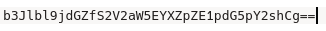
\includegraphics[width=0.7\linewidth]{files/base64}
\end{center}
\caption{То, что знакомо почти всем}
\label{fig:base64}
\end{figure}
И тут два варианта:
\begin{itemize}
\item Прогнать обратно ручками
\item Написать питоновский скрипт
\end{itemize}
Чтобы райтап был полным, рассмотрим второй вариант, потому что первый достаточно очевидный и не требует пояснений. Скрипт для расшифровки выглядит примерно следующим образом:
\newpage
\begin{lstlisting}[language=Python, caption=Дешифровка флага]
#! /usr/bin/env python3

import base65536
import pybase100 as base100
import base64

with open('flag.enc', 'r') as flag_file:
    flag = flag_file.read()

flag = base65536.decode(flag)
flag = base100.decode(flag)
flag = base64.b64decode(flag)
flag = flag.decode('utf-8')

print(flag)
\end{lstlisting}

На выходе получаем флаг \verb|oren_ctf_KevinDavidMitnick!|

%----------------------------------------------------------------------------------------

\end{document}